\documentclass[aspectratio=43,8pt]{beamer}
\usepackage[utf8]{inputenc}
%\usepackage[french]{babel}
\usepackage{multicol}
%\usepackage{basetitle}

\title{Soutenance de stage - On Demand Buffer}
\author[Brelot]{Julien Brelot}
\date{ 03 mars — 28 juillet 2025}

% Logos côte à côte sur la page de titre
% Logos sur la page de titre
\titlegraphic{%
    \includegraphics[height=2cm]{im2/logo-tps.png} \hspace{1cm}%
    
\includegraphics[height=2cm]{im2/imt.png}%
}


\usetheme{material}
\useLightTheme
\usePrimaryGreen
\useAccentCyan

\setbeamertemplate{footline}[text line]{%
  \hfill%
  \insertframenumber\,/\,\inserttotalframenumber
}

\begin{document}
%\begin{frame}
%\titlepage
%\end{frame}

\begin{frame}[plain]
    \centering
    {\Huge Soutenance de stage - On Demand Buffer\par}
    \vspace{0.5cm}
    {\large Julien Brelot\par}
    \vspace{0.5cm}
    {\large 03 mars — 28 juillet 2025\par}
    \vspace{1cm}
        \centering
        \includegraphics[width=0.45\textwidth]{img2/logo-tps.png}
        \\
        
\includegraphics[width=0.45\textwidth]{img2/imt.png}
\end{frame}

%\part{Introduction}
%    \section{Présentation du LIG}
%    \section{Contexte}
%\part{Conception d'ODB}
%    \section{Intégration dans une application existante}
%    \section{Protocole d'encapsulation}
%    \section{Messages ODB et flux de données}
%    \section{Conclusion}


\begin{frame}{Sommaire}
\tableofcontents[part=1]  % Affiche la partie 1
\tableofcontents[part=2] 
\end{frame}

\part{Introduction}

\section{Présentation du LIG}
\begin{frame}{Présentation du LIG}
\begin{card}
Le Laboratoire d’Informatique de Grenoble (LIG) est une unité mixte de recherche (UMR 5217) rattachée au CNRS, à l’Université Grenoble Alpes (UGA), à Grenoble INP et à l’Inria Grenoble Rhône-Alpes.  
Créé en 2007, il regroupe environ 500 personnes réparties sur plusieurs sites grenoblois (Saint-Martin-d’Hères, Minatec, Montbonnot).  

\medskip
\textbf{Axes de recherche principaux :}
\begin{itemize}
    \item Génie logiciel et systèmes d’information
    \item Méthodes formelles, langages et modèles
    \item Systèmes interactifs et cognitifs
    \item Calcul parallèle, distribué et réseaux
    \item Traitement des données massives et gestion des connaissances
\end{itemize}
\end{card}
\end{frame}

\begin{frame}{L’équipe KrakOS}
\begin{card}
Créée en octobre 2024, KrakOS (Optimiser les couches système des centres de données) est spécialisée dans les systèmes d’exploitation, environnements virtualisés et middlewares cloud.  
L’équipe, dirigée par Alain Tchana, regroupe enseignants-chercheurs, doctorants et ingénieurs de recherche.

\medskip
\textbf{Objectifs de KrakOS :}
\begin{enumerate}
    \item Améliorer les performances des systèmes (temps d’exécution, débit, latence)
    \item Renforcer tolérance aux pannes et haute disponibilité
    \item Faciliter le développement, tests et déploiement rapide
    \item Fournir des API expressives et flexibles aux développeurs
    \item Réduire la consommation énergétique des infrastructures
\end{enumerate}

\medskip
KrakOS bénéficie d’un environnement scientifique riche, avec des collaborations nationales et internationales (ex. IRISA, IRIT).
\end{card}
\end{frame}

\section{Contexte}
\begin{frame}{Contexte Général (1/3)}
    \begin{card}
        \begin{itemize}
            \item Les \textbf{datacenters} et le \textbf{cloud computing} sont au cœur des infrastructures modernes, hébergeant services en ligne critiques : e-commerce, banques, messagerie, réseaux sociaux.
            \item Les applications suivent souvent des architectures \textbf{multi-tiers} : 
            \begin{itemize}
                \item \emph{Front-end} : présentation / point d'entrée,
                \item \emph{Middle-tier} : logique métier,
                \item \emph{Back-end} : gestion des données.
            \end{itemize}
            \item Cette séparation assure modularité, maintenabilité et scalabilité.
        \end{itemize}
    \end{card}
\end{frame}

\begin{frame}{Contexte Général (2/3)}
    \begin{card}
        \begin{itemize}
            \item \textbf{Problèmes majeurs des architectures multi-tiers :}
            \begin{itemize}
                \item Multiplication des \textbf{copies de données} : buffers applicatifs, mémoire noyau, transferts réseau → utilisation inefficace CPU et bande passante.
                \item \textbf{Backpressure} : accumulation de buffers lorsque les couches amont produisent plus vite que les couches aval peuvent traiter → augmentation de latence.
                \item Opérations \textbf{I/O} coûteuses : appels système, basculement mode utilisateur/noyau, copies multiples → saturent CPU et bus mémoire.
            \end{itemize}
        \end{itemize}
    \end{card}
\end{frame}

\begin{frame}{Contexte Général (3/3)}
    \begin{card}
        \begin{itemize}
            \item Objectif du projet : optimiser les performances des architectures multi-tiers dans le cloud.
            \item Solution proposée : \textbf{On-Demand Buffer (ODB)}
            \begin{itemize}
                \item Détecte de façon transparente l’usage réel des données par les intermédiaires.
                \item Transfère uniquement les données nécessaires, réduisant les copies inutiles.
                \item Mitige la contre-pression et améliore la performance I/O.
            \end{itemize}
            \item Bénéfices attendus : réduction CPU, réduction latence, meilleur débit et meilleure utilisation des ressources pour les applications modernes.
        \end{itemize}
    \end{card}
\end{frame}

\begin{frame}{Contexte : Illustration}
\centering
\cardImg{img/problem.png}{\textwidth}
\end{frame}

\part{Conception d'ODB}

\section{Intégration dans une application existante}
\begin{frame}{Intégration dans une application existante}
\begin{itemize}
    \item \textbf{Objectif d'ODB} : fonctionner avec une application web existante sans modifier le code source.
    \item Contraintes clés :
    \begin{itemize}
        \item Ne pas perturber les communications existantes (HTTP, FTP, SMTP…).
        \item Envoyer et recevoir des données, sans bloquer l'application.
        \item Séparer les données ODB des buffers de l'application.
        \item Gérer les erreurs ODB sans impacter l'application.
    \end{itemize}
    \item Nécessité de \textbf{sockets connectées et séquentielles} (TCP) pour garantir la cohérence des échanges.
\end{itemize}
\end{frame}

\section{Alignement des données}

\begin{frame}{Alignement des données}
\begin{itemize}
    \item ODB utilise \texttt{mprotect()} pour protéger l'accès aux données.
    \item \textbf{Contraintes de mprotect} :
    \begin{itemize}
        \item Protection à la granularité d'une page.
        \item Mémoire alignée sur les frontières de pages.
    \end{itemize}
    \item Buffers non-alignés :
    \begin{itemize}
        \item \textbf{Head} : début non aligné (< page)
        \item \textbf{Body} : zone alignée et multiple d'une page
        \item \textbf{Tail} : fin non alignée (< page)
    \end{itemize}
    \item Données Head/Tail doivent être transférées "réellement", Body peut rester virtualisé.
\end{itemize}
\begin{figure}
    \centering
    \includegraphics[scale=0.4]{img2/memory_pb.png}
    \caption{Zones mémoire Head / Body / Tail}
\end{figure}
\end{frame}

\section{Protocole d'encapsulation}
\begin{frame}{Protocole d'encapsulation}
\begin{itemize}
    \item Besoin : garantir la cohérence et la compatibilité avec POSIX malgré les non-alignements.
    \item Solution : \textbf{protocole d'encapsulation ODB} 
    \begin{itemize}
        \item En-tête \texttt{ODB\_Header} : type de données (réelles ou virtuelles)
        \item Pour les données virtuelles : \texttt{ODB\_Desc} décrit Body/Head/Tail et back-end
        \item Interception des appels système pour ajouter/extraire ces informations au niveau applicatif
    \end{itemize}
    \item Nécessité de sockets séquentielles pour traiter les en-têtes ODB avant les données applicatives.
\end{itemize}
\begin{figure}
    \centering
    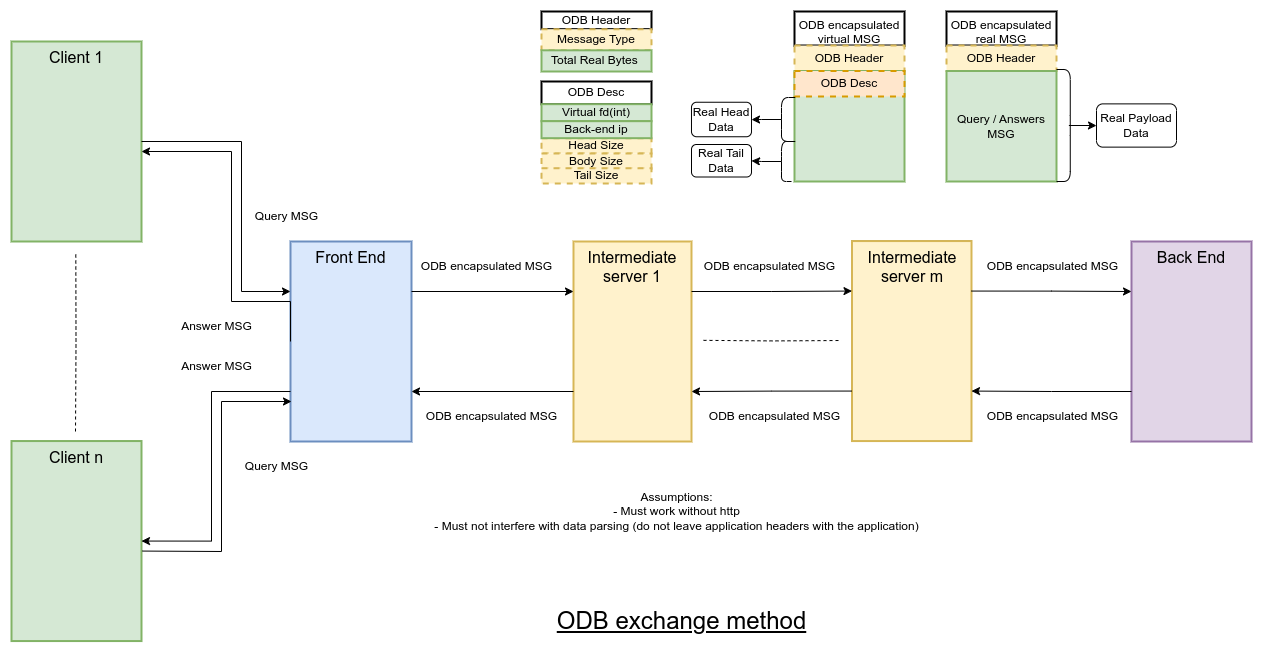
\includegraphics[scale=0.3]{img2/odb_communication.png}
    \caption{Communication et encapsulation ODB}
\end{figure}
\end{frame}


\section{Messages ODB et flux de données}
\begin{frame}{Messages ODB et flux de données}
\begin{itemize}
    \item Messages ODB contiennent :
    \begin{itemize}
        \item Identifiant virtuel de la page, IP/port back-end
        \item Tailles des zones Head, Body, Tail
    \end{itemize}
    \item Données virtualisées vs données réelles :
    \begin{itemize}
        \item Head/Tail : transférées effectivement
        \item Body : virtualisé, transfert à la demande
    \end{itemize}
    \item Objectif : transparence totale pour l'application, cohérence des échanges garantie.
\end{itemize}
\begin{figure}
    \centering
    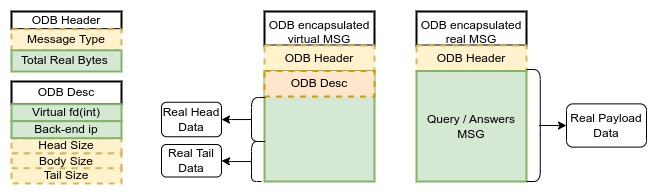
\includegraphics[scale=0.3]{img2/odb_c_messages.jpg}
    \caption{Détail des messages ODB}
\end{figure}
\end{frame}


\part{Réalisation Technique}
\section{Utilisation du protocole ODB}
\begin{frame}{Utilisation du protocole ODB}
\begin{itemize}
    \item ODB nécessite que \textbf{les deux applications} utilisent le protocole pour garantir la cohérence des échanges.
    \item Deux approches pour gérer l’activation d’ODB :
    \begin{enumerate}
        \item Fichier de configuration : indique les ports où ODB est actif.
        \item Mode \emph{stand-alone} : détection automatique via un \emph{magic number} + CRC-8.
    \end{enumerate}
    \item Objectif : permettre au front-end de communiquer correctement avec le back-end ODB tout en restant compatible avec des clients classiques.
\end{itemize}
\end{frame}

\section{Gestion des buffers non-alignés}
\begin{frame}{Gestion des buffers non-alignés}
\begin{itemize}
    \item Head/Tail : parties non-alignées, transmises en données réelles.
    \item Body : zone alignée, peut rester virtualisée.
    \item Stratégies d’envoi :
    \begin{itemize}
        \item \textbf{Statique} : taille fixe (\emph{unaligned\_size}), simple mais limite l’hétérogénéité.
        \item \textbf{Dynamique} : taille variable, téléchargement à la demande depuis le BE.
        \item \textbf{Anticipation} : hybride, BE envoie Head/Tail vers le IS suivant pour réduire les requêtes.
    \end{itemize}
    \item Gestion des buffers de réception insuffisants : téléchargement segmenté Head/Body/Tail et maintien de l’état de réception.
\end{itemize}
\begin{figure}
    \centering
    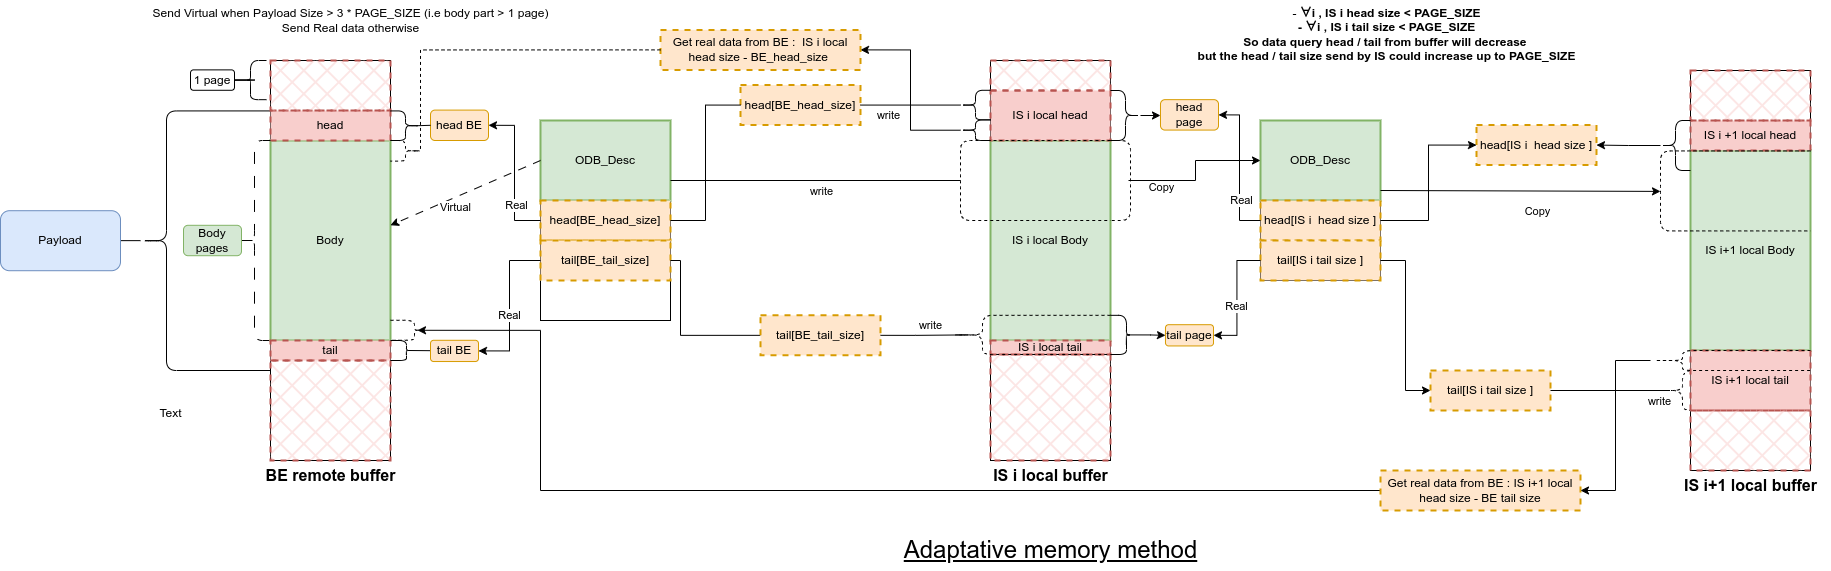
\includegraphics[width=0.7\textwidth]{img/odb_adaptative_memory.png}
    \caption{Stratégie d'anticipation pour buffers non-alignés}
\end{figure}
\end{frame}

\section{Développement de serveurs tests}
\begin{frame}{Développement de serveurs tests}
\begin{itemize}
    \item Objectif : tester et déboguer ODB.
    \item Composants :
    \begin{itemize}
        \item FE : envoie des requêtes et reçoit des fichiers.
        \item IS : transfère les données entre BE et FE.
        \item BE : lit le fichier et envoie les données au FE via les IS.
    \end{itemize}
    \item Paramétrable via flags pour tester différentes tailles de buffers.
    \item Application cible pour tests réels : \textbf{nginx}, serveur web/ reverse-proxy majoritairement utilisé.
\end{itemize}
\end{frame}

\section{Utilisation avec Nginx}
\begin{frame}{Utilisation avec Nginx}
\begin{itemize}
    \item Nginx utilise plusieurs processus :
    \begin{itemize}
        \item Master : gestion configuration et processus
        \item Cache Loader / Manager : gestion mémoire cache
        \item Worker : boucle événementielle pour traiter les connexions
    \end{itemize}
    \item Boucle d’événements :
    \begin{itemize}
        \item Surveillance des descripteurs (epoll/poll/kqueue)
        \item Traitement séquentiel des événements
        \item Sockets non-bloquantes nécessaires
    \end{itemize}
    \item Thread pools pour gérer I/O lourdes sans bloquer les workers.
\end{itemize}
\begin{figure}
    \centering
    \includegraphics[width=0.6\textwidth]{img2/nginx-event-Loop.png}
    \caption{Boucle événementielle des workers Nginx}
\end{figure}
\end{frame}

\begin{frame}{Problème avec epoll Edge Triggered (5/5)}
\begin{itemize}
    \item Mode Edge Triggered : notification seulement lors du changement d’état de la socket.
    \item Problème : ODB virtualise les données, Nginx peut ne pas lire tout le buffer restant.
    \item Solutions envisagées :
    \begin{enumerate}
        \item Vérifier après chaque \textit{recv} et forcer un événement EPOLLIN si nécessaire.
        \item Intercepter \textit{epoll\_create} et \textit{epoll\_ctl} pour passer en mode Level Triggered.
    \end{enumerate}
    \item Conséquence : complexité accrue et risque de latence supplémentaire sur la boucle événementielle.
    \item Conclusion : intégration ODB dans Nginx nécessite de gérer finement la lecture/écriture sur sockets pour éviter les pertes de données.
\end{itemize}
\end{frame}


\section{Résultats et analyse}

\begin{frame}{Tests menés}
\begin{itemize}
    \item 3 serveurs Nginx sur 3 nœuds Grid5000, 1 worker par serveur, 1 cœur logique.
    \item Front-end et serveur intermédiaire : 2 proxies ; back-end : serveur HTTP.
    \item Proxy buffering désactivé.
    \item Charge : 50 clients/s jusqu'à 1000 clients, ~30k requêtes GET.
    \item Payloads virtuelles : \{16, 32, 64, 128, 256 Ko\}.
    \item Métriques : CPU total, CPU sur cœur du worker, mémoire, latence et débit.
    \item Variables : alignement des buffers, stratégie ODB (\textit{dynamic} vs \textit{anticipated}).
\end{itemize}
\end{frame}

\begin{frame}{ODB : Stratégies d'envoi (non-aligné)}
\begin{itemize}
    \item \textit{dynamic} vs \textit{anticipated}.
    \item CPU similaire pour FE, IS, BE.
    \item IS : gain notable à partir de 128 Ko avec \textit{dynamic}.
    \item Latence légèrement meilleure avec \textit{anticipated}, surtout pour grosses payloads.
    \item Choix retenu : \textit{dynamic} pour réduire CPU.
\end{itemize}
\begin{figure}
    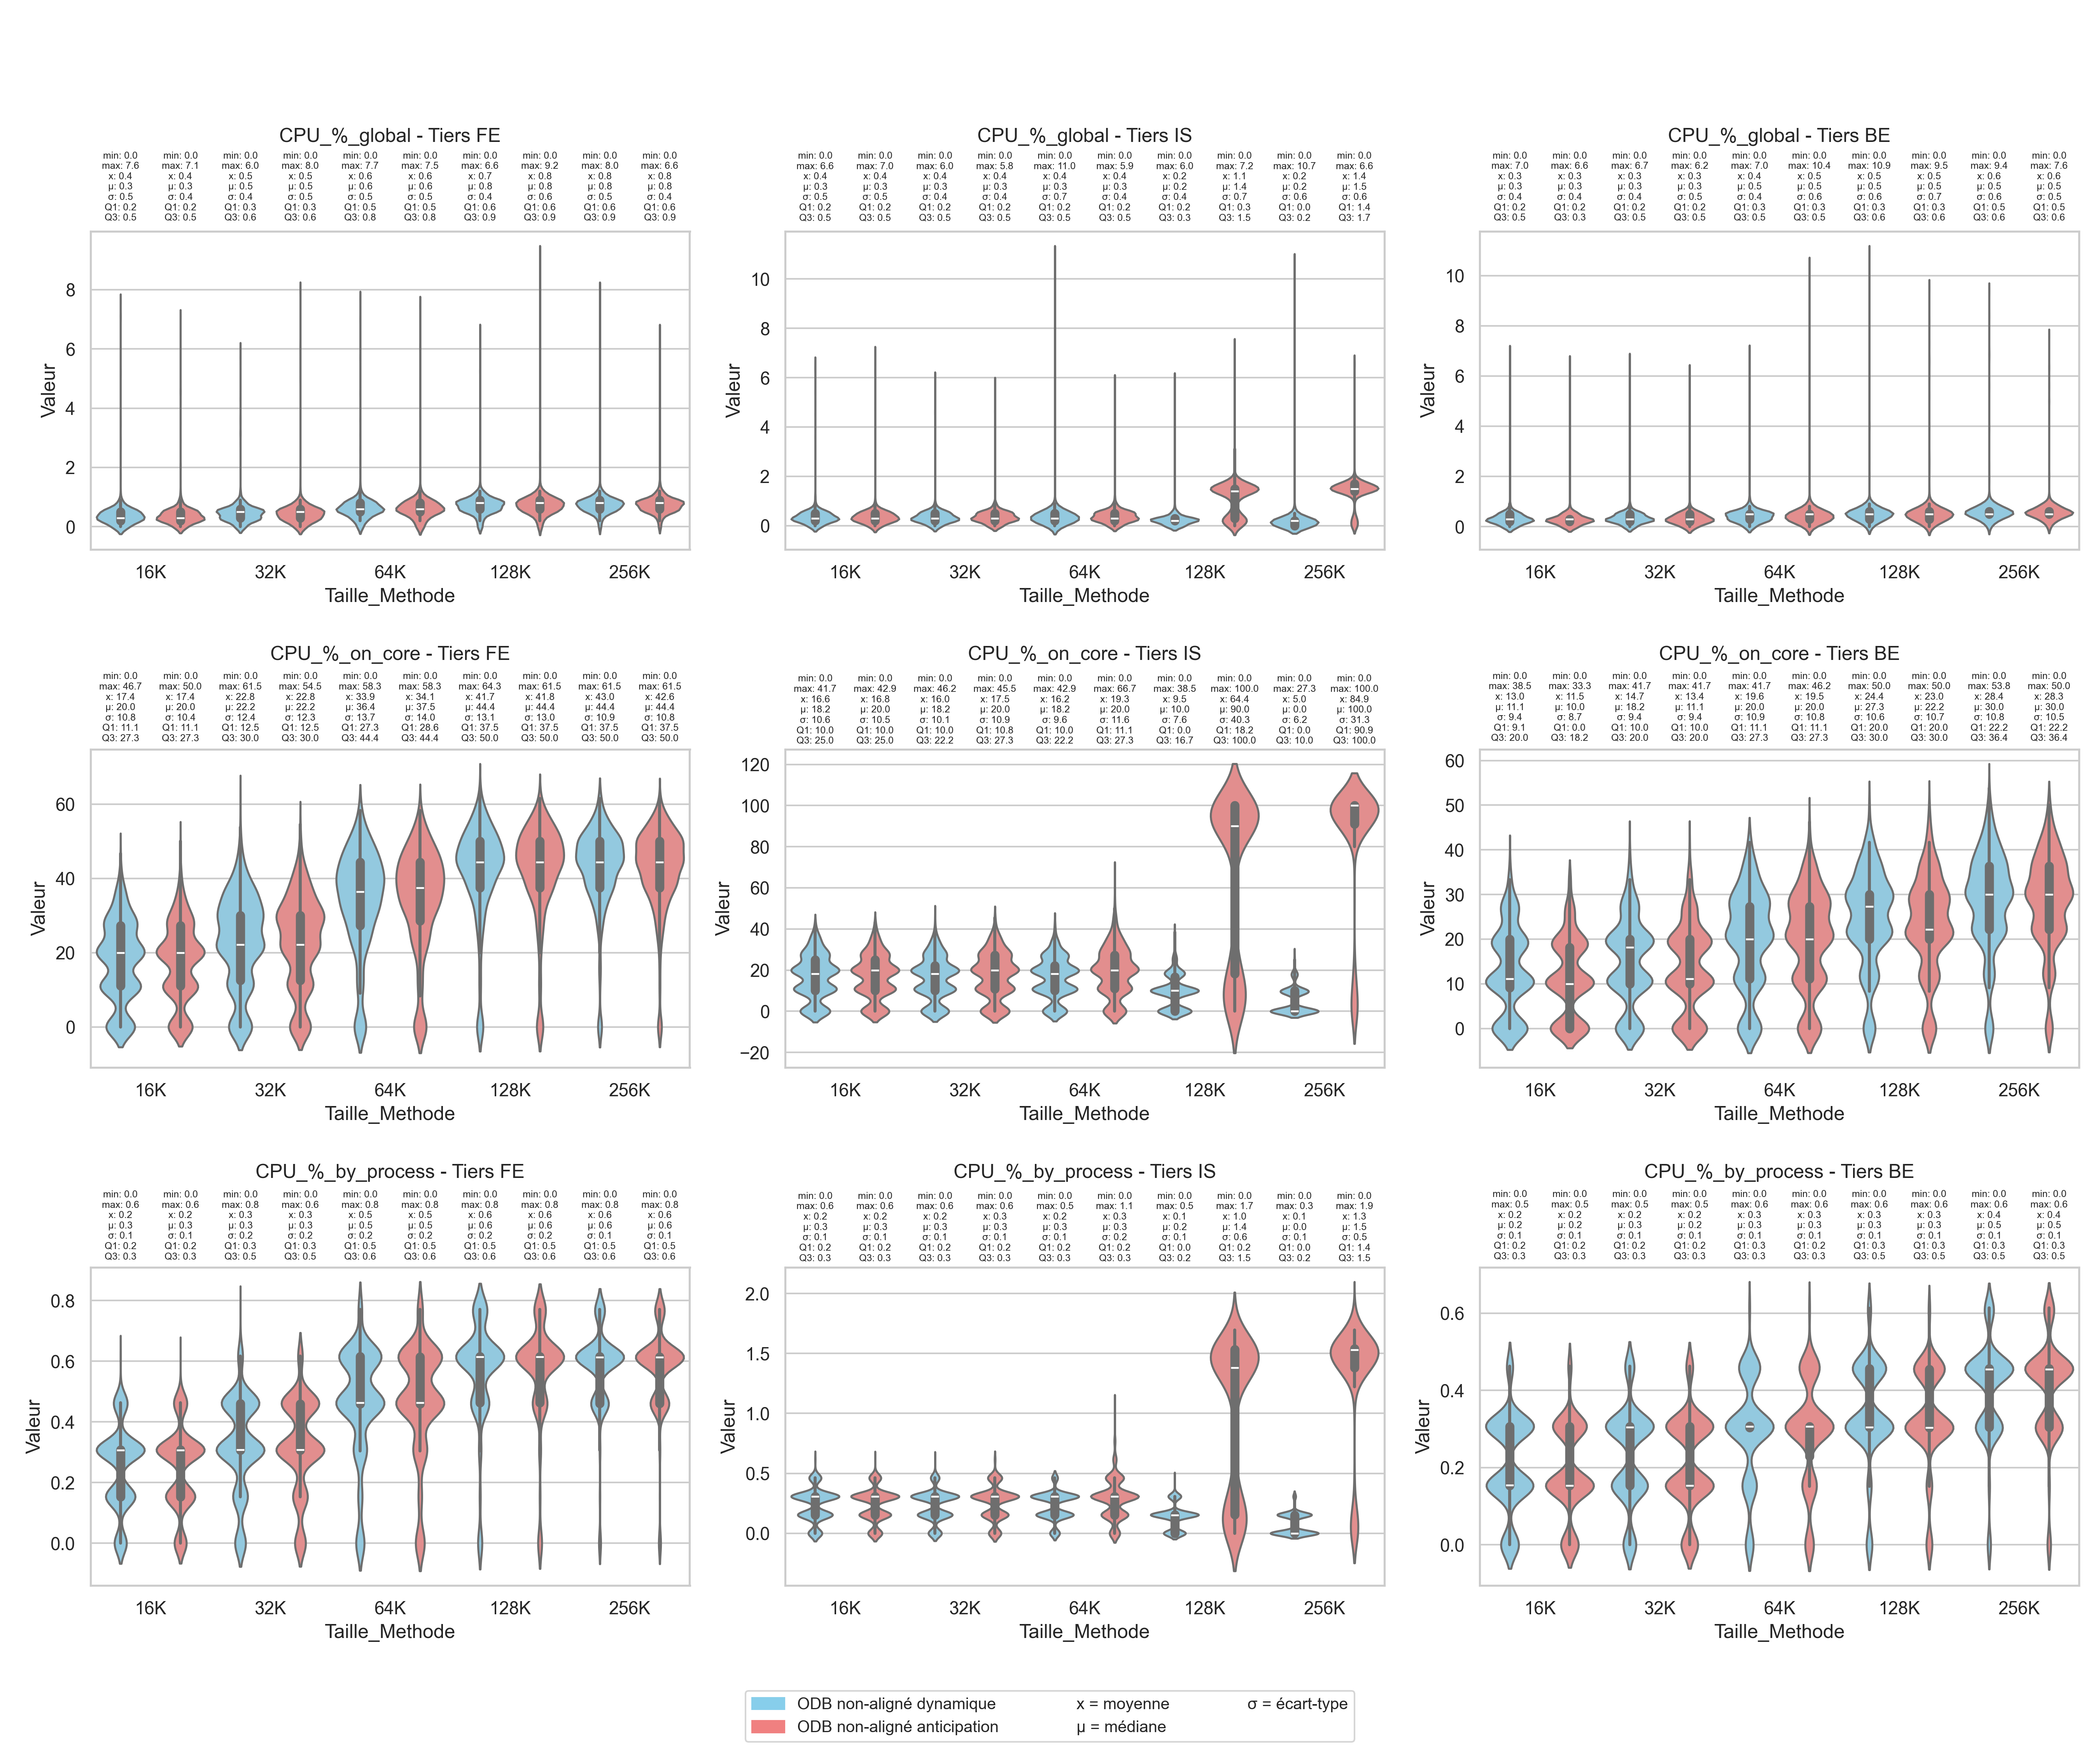
\includegraphics[width=\textwidth]{results/results-cmp/odb_unaligned_dynamic_vs_anticipated.png}
\end{figure}
\end{frame}

\begin{frame}{ODB : Alignement vs non-alignement (dynamic)}
\begin{itemize}
    \item Alignement peu impactant à faible payload.
    \item 128-256 Ko : réduction CPU sur FE et BE.
    \item Latence moyenne comparable mais légère amélioration pour grosses payloads.
    \item Explication : réduction des requêtes pour head/tail des buffers.
\end{itemize}
\begin{figure}
    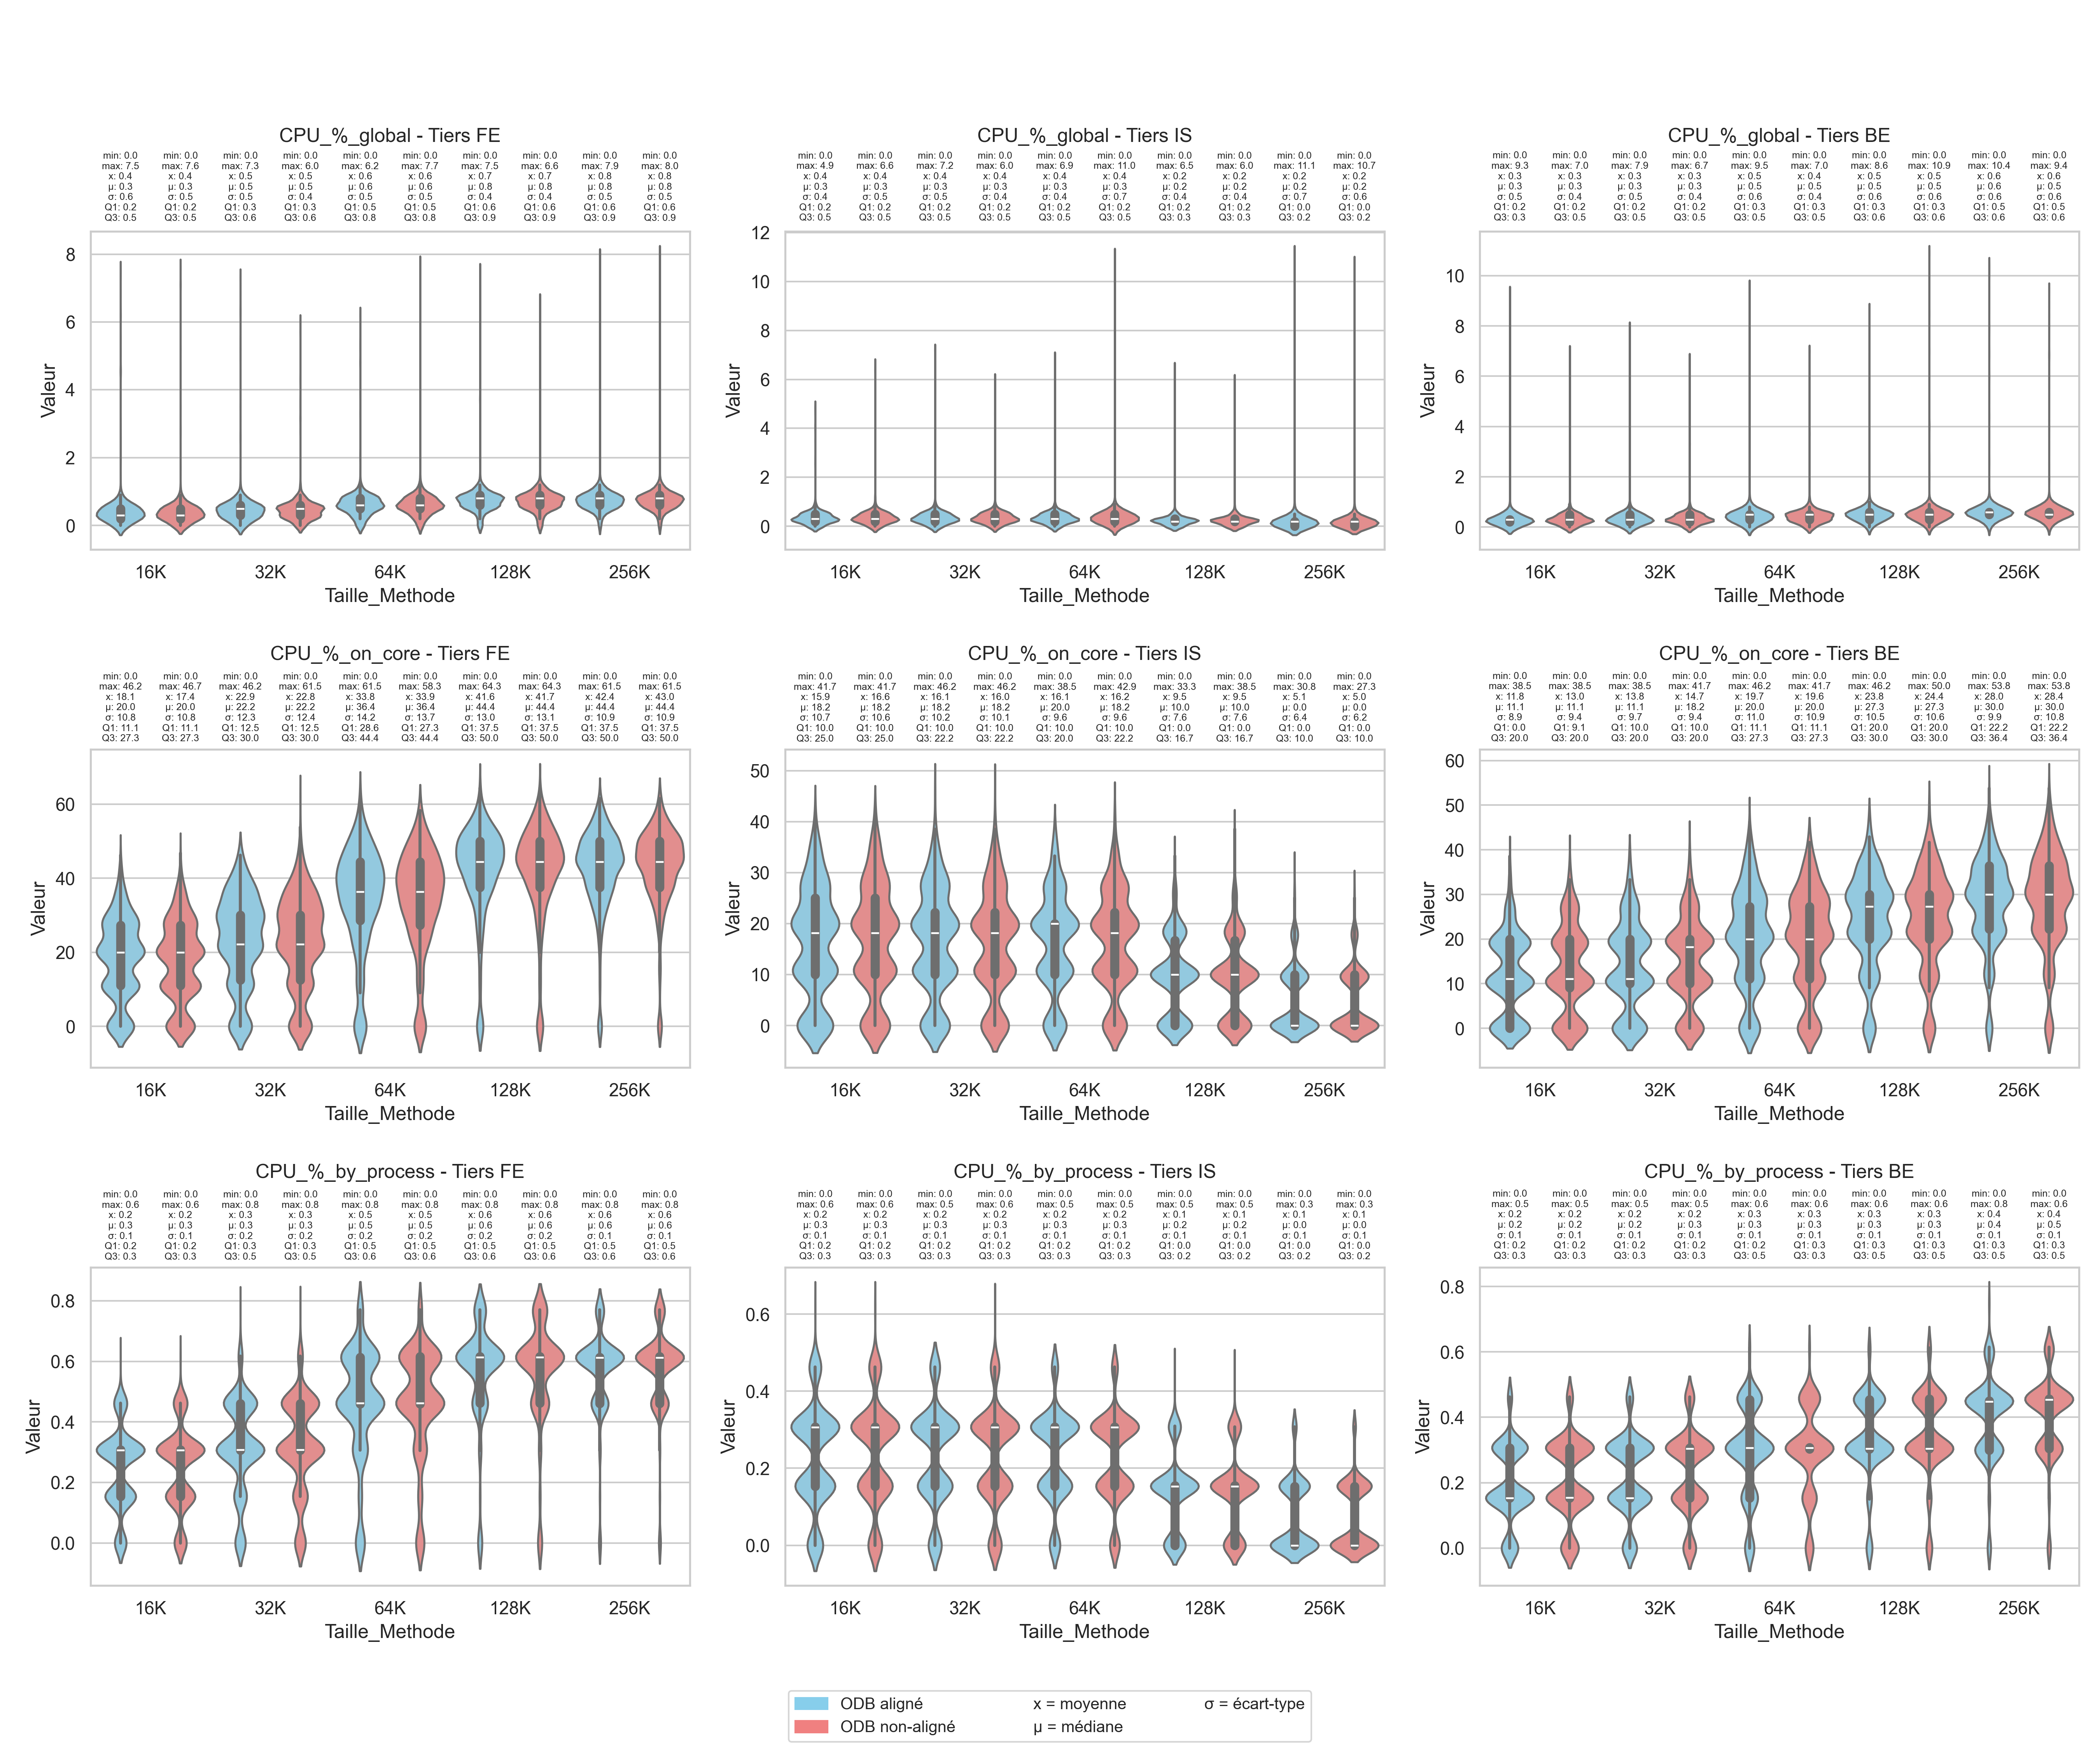
\includegraphics[width=\textwidth]{results/results-cmp/odb_aligned_vs_unaligned_dynamic.png}
\end{figure}
\end{frame}

\begin{frame}{Vanilla : Alignement vs non-alignement}
\begin{itemize}
    \item Pas d'impact notable sur CPU ou QOS.
    \item Alignement user-space ignoré par le kernel lors des écritures sur socket.
\end{itemize}
\begin{figure}
    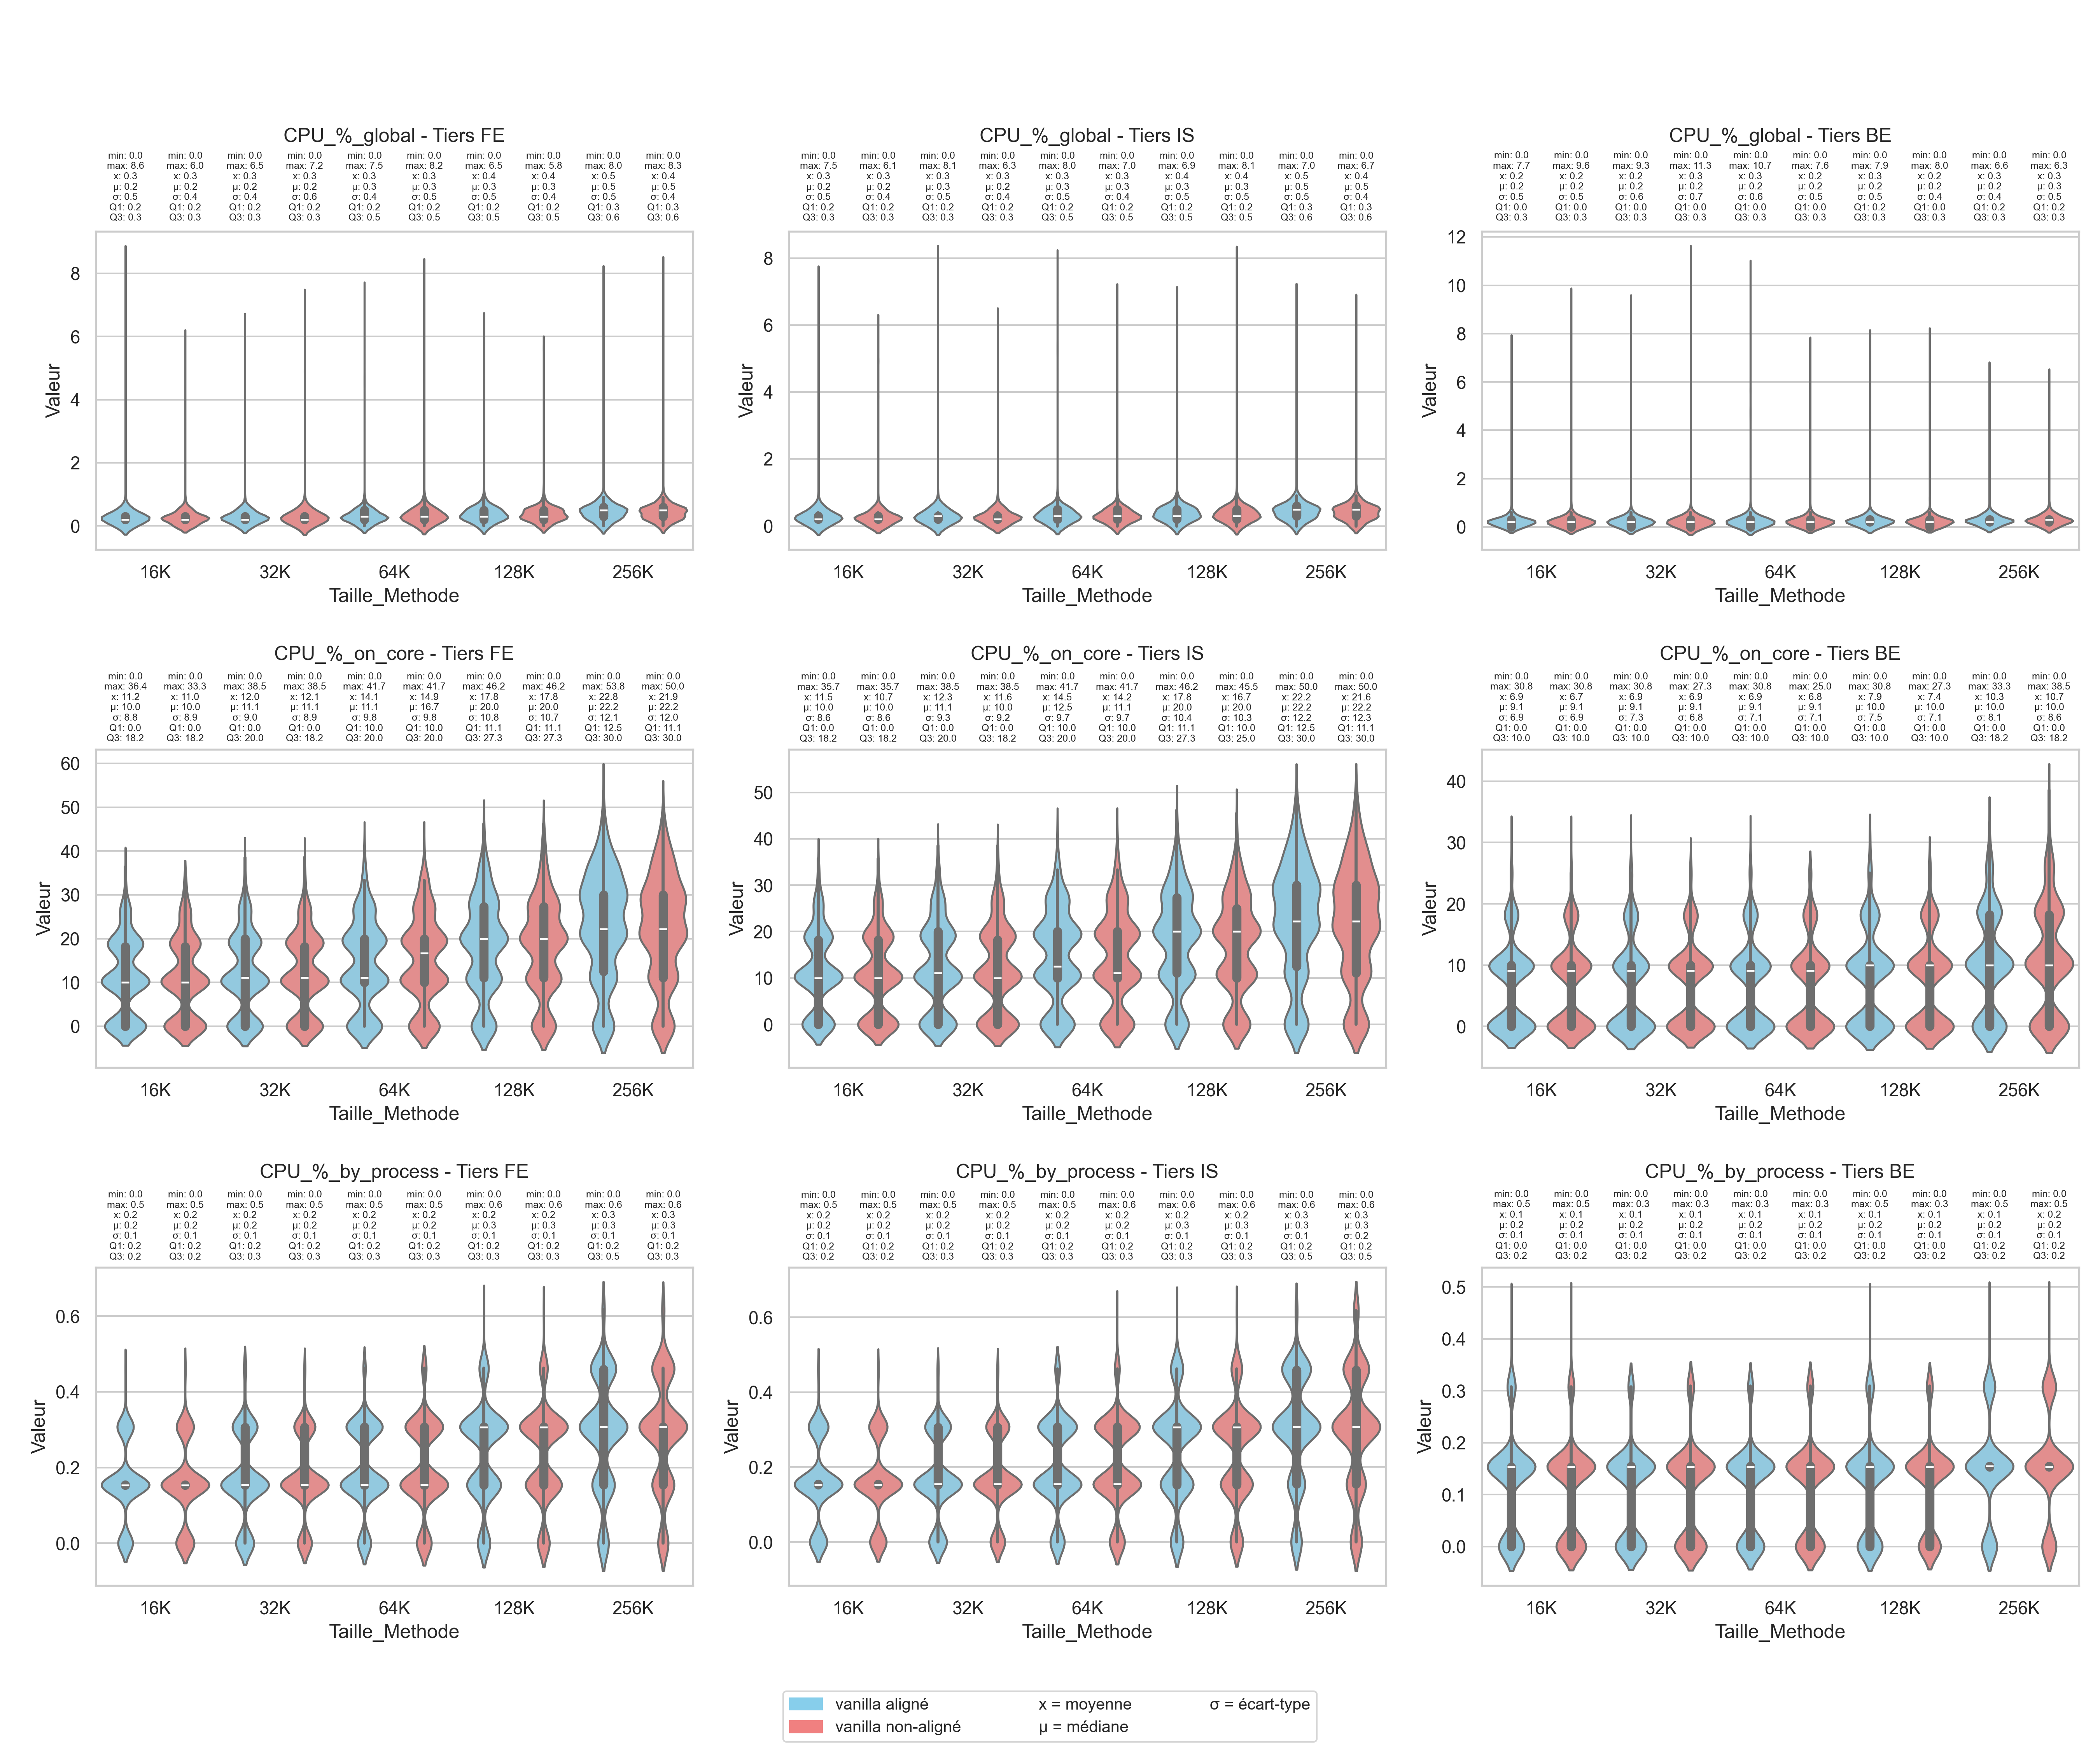
\includegraphics[width=\textwidth]{results/results-cmp/vanilla_aligned_vs_unaligned.png}
\end{figure}
\end{frame}

\begin{frame}{ODB vs Vanilla (aligné)}
\begin{itemize}
    \item IS : réduction CPU notable pour payloads > 128 Ko.
    \item FE et BE : augmentation CPU (BE double pour 256 Ko).
    \item Latence ODB > Vanilla, surtout pour grosses payloads.
    \item Explication : sockets bloquantes pour transfert de payload virtuelle.
\end{itemize}
\begin{figure}
    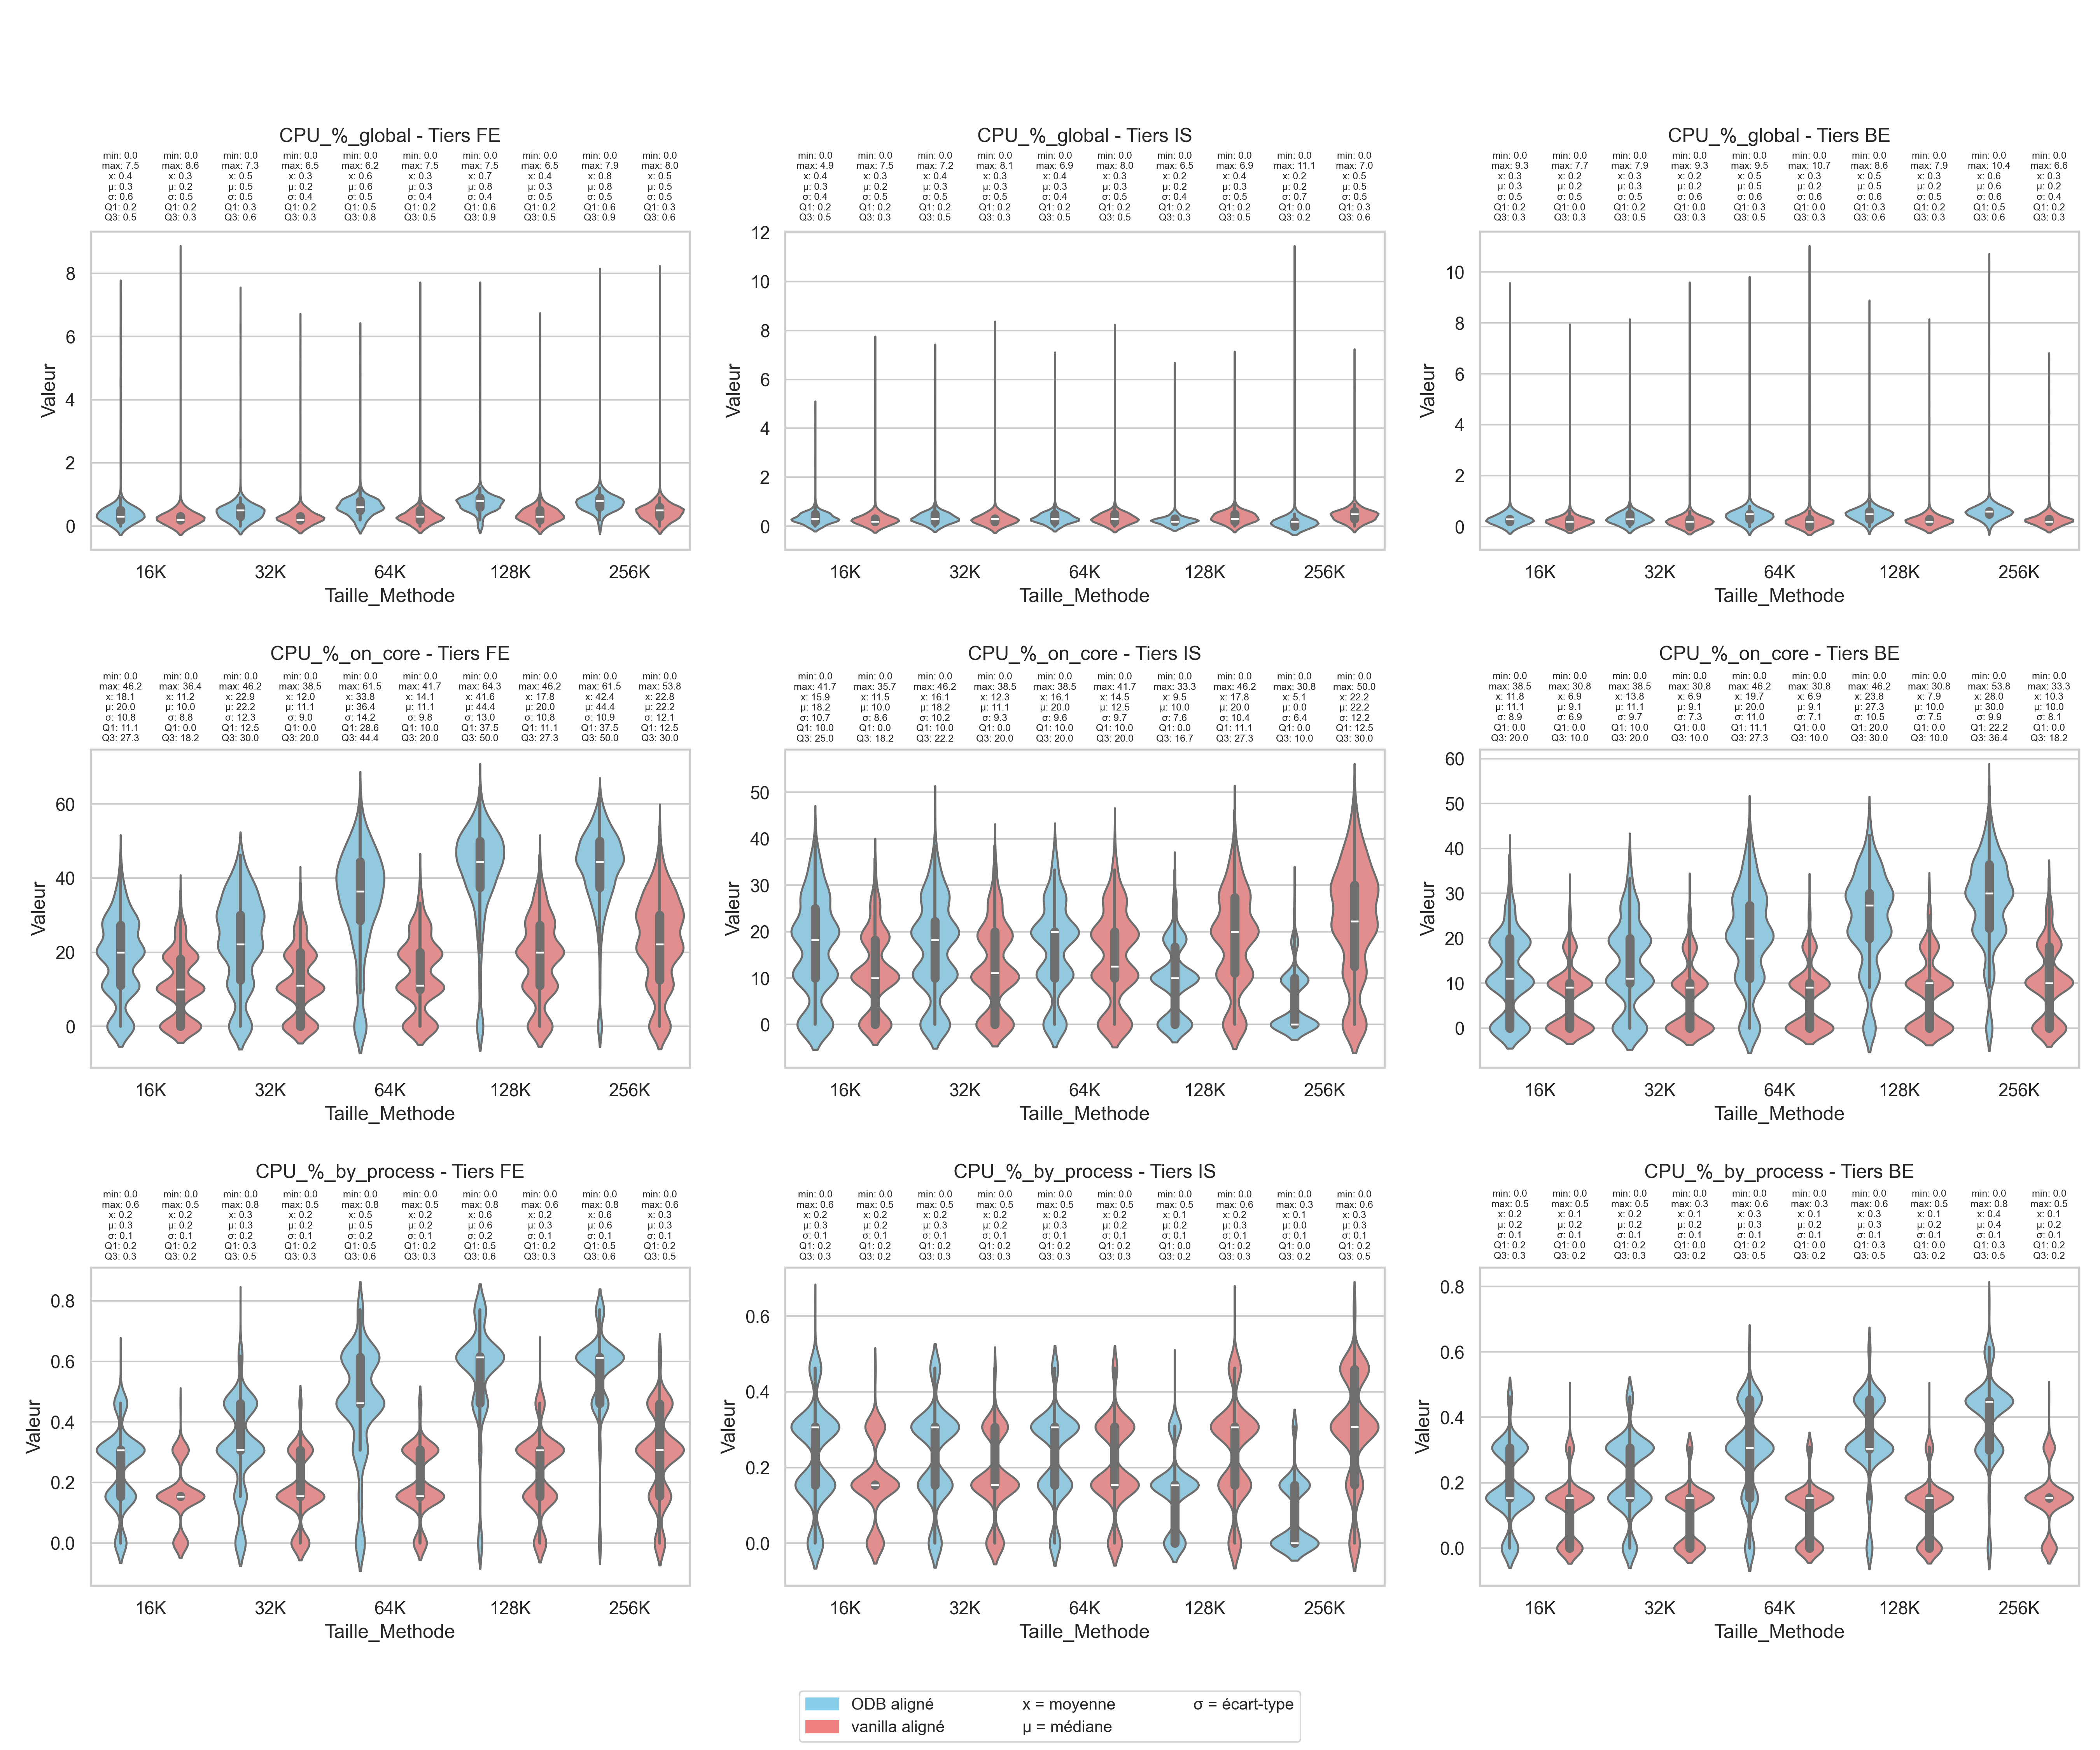
\includegraphics[width=\textwidth]{results/results-cmp/odb_dynamic_vs_vanilla_aligned.png}
\end{figure}
\end{frame}

\begin{frame}{ODB vs Vanilla (non-aligné)}
\begin{itemize}
    \item Tendances similaires à l'aligné.
    \item Écart CPU FE/BE plus important : overhead head/tail.
    \item IS : réduction CPU pour grosses payloads.
    \item Latence : ODB plus élevée, même tendance que pour aligné.
\end{itemize}
\begin{figure}
    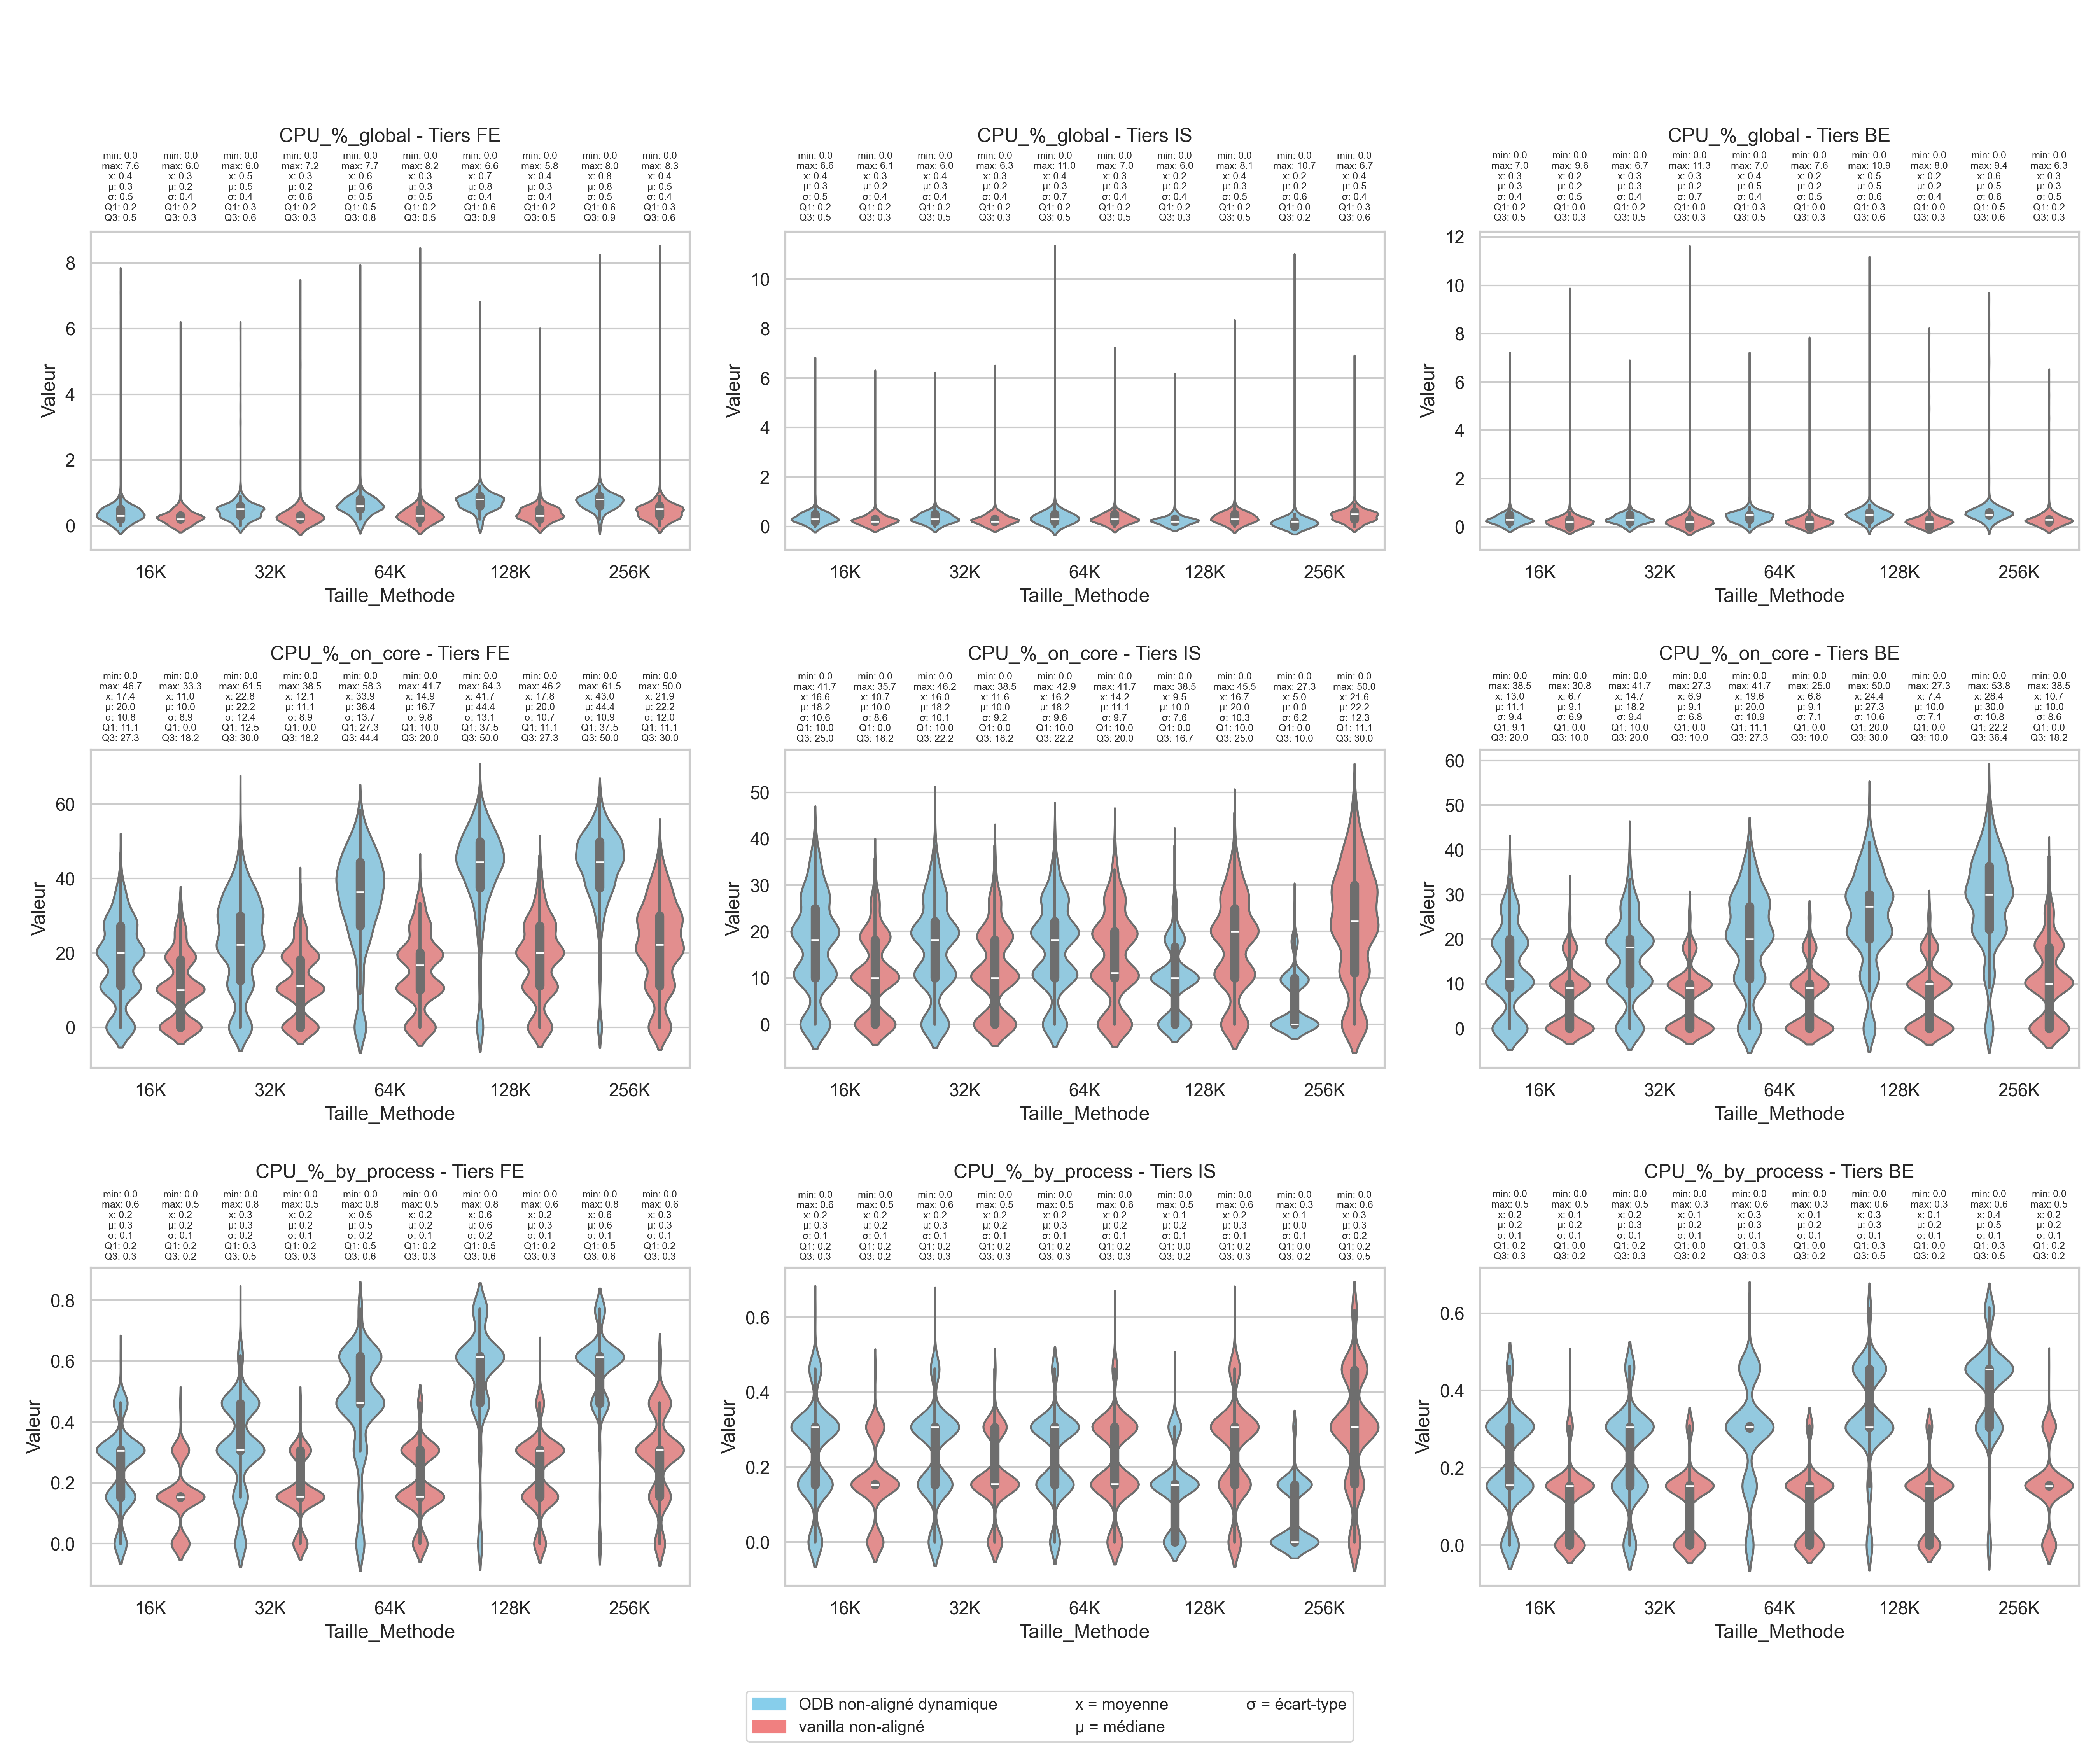
\includegraphics[width=\textwidth]{results/results-cmp/odb_dynamic_vs_vanilla_unaligned.png}
\end{figure}
\end{frame}

\section{Problème de téléchargement indisponible}
\begin{frame}{Problème : téléchargement indisponible}
\begin{itemize}
    \item Payload virtuelle : téléchargement depuis BE uniquement à la demande.
    \item Problème : BE inaccessible → SIGSEGV ou données corrompues.
    \item Solutions envisagées :
    \begin{enumerate}
        \item Arrêt du processus
        \item Corruption contrôlée
        \item Envoi simulé
        \item Best-effort (retransmission si possible)
    \end{enumerate}
\end{itemize}
\begin{figure}
    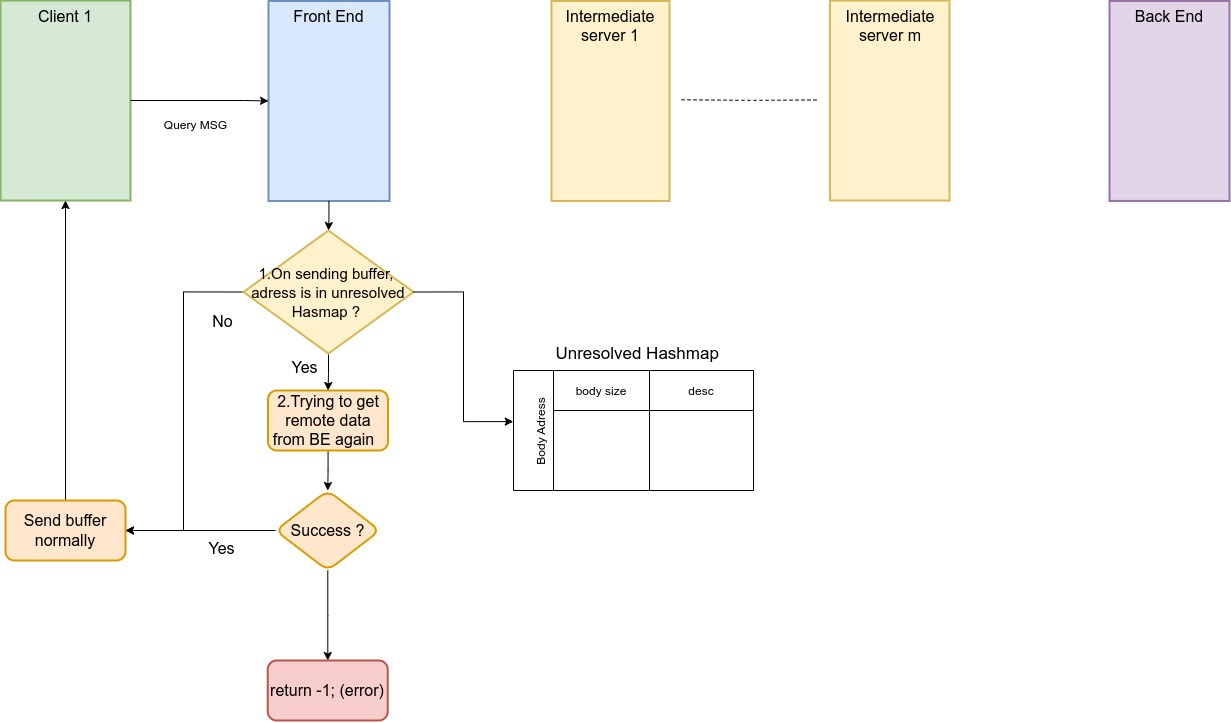
\includegraphics[width=\textwidth]{img2/odb_c_best_effort.jpg}
\end{figure}
\end{frame}

\section{Problème d'utilisation mémoire pour les buffers virtuels}
\begin{frame}{Problème : utilisation mémoire pour buffers virtuels}
\begin{itemize}
    \item Chaque payload virtuelle allouée en mémoire du BE.
    \item Plus de requêtes → plus de mémoire utilisée.
    \item Solution : ramasse-miettes :
    \begin{itemize}
        \item Supprime payloads virtuelles utilisées
        \item Thread dédié supprime payloads non utilisées après un délai configurable
    \end{itemize}
\end{itemize}
\end{frame}


\part{Conclusion}
\begin{frame}{Conclusion et perspectives (1/2)}
\begin{itemize}
    \item \textbf{ODB} : idée originale et prometteuse pour réduire l'envoi de données redondantes.
    \item Réduction potentielle de la charge CPU, consommation réseau et énergétique.
    \item Limites observées :
    \begin{itemize}
        \item Surcoût CPU et latence liés à l'utilisation de \textit{mprotect}.
        \item Augmentation de la latence globale par rapport à vanilla, réduisant la QoS.
        \item Charge transférée du serveur intermédiaire vers le Back-End et Front-End.
    \end{itemize}
    \item Protocole pertinent pour un usage plus écologique et plus respectueux de l’environnement.
\end{itemize}
\end{frame}

\begin{frame}{Conclusion et perspectives (2/2)}
\begin{itemize}
    \item \textbf{Pistes d’amélioration :}
    \begin{itemize}
        \item Explorer l’utilisation de \textit{userfaultfd} pour remplacer \textit{mprotect}.
        \item Étudier l’intégration de sockets non-bloquantes pour exploiter la boucle d’événements de nginx.
        \item Développer une API dédiée pour limiter les détournements de fonctions \textit{libc} et améliorer les performances.
    \end{itemize}
    \item Ces axes pourraient réduire les impacts des limitations actuelles et améliorer la portabilité et l’efficacité d'ODB.
\end{itemize}
\end{frame}


\begin{frame}[noframenumbering]{Repo git}
\begin{figure}[h]
    \centering
    \href{https://github.com/BJCode-git/ODB-C}{%
        
\includegraphics[scale=1]{img2/github-mark.png}%
    }
    \caption{Lien vers mon repo GitHub}
    \label{fig:github}
\end{figure}
\end{frame}


\end{document}

%
%
%\begin{frame}{ODB : Principes}
%\centering
%\cardImg{img/odb_1.png}{0.8\textwidth}
%\begin{card}
%    \begin{itemize}
%        \item   Le Back-End (BE) envoie les données de manière "virtuelle"
%        \item   Les données virtuelles contiennent l’IP et le descripteur de fichier virtuel du Back-End
%        \item   Enfin, si aucun SI n’a eu besoin de traiter la réponse, le FE téléchargera les données directement depuis le BE
%    \end{itemize}
%\end{card}
%\end{frame}
%
%\begin{frame}{ODB : Principes}
%\centering
%\cardImg{img/odb_2.png}{0.8\textwidth}
%\begin{card}
%Si un SI doit traiter les données :
%    \begin{itemize}
%        \item   Il téléchargera les données depuis le BE
%        \item   Il traitera les données et les enregistrera localement
%        \item   Il se comportera ensuite comme un BE pour ces données
%    \end{itemize}
%\end{card}
%\end{frame}
%
%\begin{frame}{Enjeux à haut niveau}
%\centering
%\begin{card}
%    \begin{itemize}
%        \item   Détecter quand les données sont accédées
%        \item   Télécharger les données lors de l’accès mémoire
%        \item   Éviter de reformater le code existant
%        \item   Ne pas interférer avec le processus de l’application
%        \item   Nous supposerons une charge utile monolithique
%    \end{itemize}
%\end{card}
%\end{frame}
%
%\begin{frame}{Enjeux techniques}
%
%\begin{card}
%    \begin{itemize}
%        \item   Les données ne sont pas forcément alignées par page, ce qui laisse certaines données non protégées
%        \item   Le FE doit savoir qu’il doit télécharger et envoyer les données réelles au client
%    \end{itemize}
%\end{card}
%\begin{figure}[ht]
%        \centering
%        \includegraphics[scale=0.5]{img/memory_pb.png}
%        \caption{Alignement mémoire}
%        \label{fig:memory_pb}
%    \end{figure}
%\end{frame}
%
%
%\begin{frame}{Approche ODB : Communication}
%\begin{card}
%    \begin{itemize}
%        \item   Encapsuler les données avec un en-tête ODB
%        \item   Identifier si la connexion est ODB ou non
%        \item   Fournir des informations sur les données (taille)
%    \end{itemize}
%\end{card}
%\end{frame}
%
%\begin{frame}{Approche ODB : Communication (2)}
%\centering
%\cardImg{img/odb_communication.png}{\textwidth}
%\end{frame}
%
%
%\begin{frame}{Approche ODB : Gestion du désalignement mémoire (1)}
%\begin{card}
%    \begin{itemize}
%        \item   Les parties tête/queue ne dépassent jamais une taille spécifiée S
%        \item   Envoyer les S premiers octets (tête) et les S derniers octets (queue) pour l’envoi virtuel
%        \item   Envoyer un descripteur virtuel à la place de la partie principale de la charge utile
%        \item   Le descripteur sera protégé dans la partie principale
%        \item   Si la taille de la charge utile est inférieure à une taille spécifiée, envoyer les données réelles
%    \end{itemize}
%\end{card}
%\end{frame}
%
%\begin{frame}{Approche ODB : Gestion du désalignement mémoire (2)}
%\centering
%\cardImg{img/odb_simple_memory.png}{\textwidth}
%\end{frame}
%
%\begin{frame}{Approche ODB : Gestion du désalignement mémoire (3)}
%\begin{card}
%    \begin{itemize}
%        \item   Les parties tête/queue ne dépassent jamais une taille spécifiée S
%        \item   Chaque SI propage les parties tête/queue acquises jusqu’à présent
%        \item   Si les données reçues ne suffisent pas à compléter la tête/queue locale, les obtenir depuis le Back-End
%    \end{itemize}
%\end{card}
%\end{frame}
%
%\begin{frame}{Approche ODB : Gestion du désalignement mémoire (4)}
%\centering
%\cardImg{img/odb_adaptative_memory.png}{\textwidth}
%\end{frame}%